%========================================================================
%
%========================================================================
\section{Des exemples}

   Le répertoire {\tt examples} des sources de {\sc ndes} comprend un
certain nombre d'exemples. Certains de ces exemples servent de
tutoriels et ont donc été décrits précédemment. D'autres sont
présentés ici.

%------------------------------------------------------------------------
%
%------------------------------------------------------------------------
\subsection{Modélisation des sources}
\label{subsection:trafic-base}

   Dans un simulateur réseau, la modélisation des sources de trafic
joue un rôle particulièrement important. Ce sont en effet les sources
qui induisent le trafic et sont donc à l'origine de la dynamique du
réseau.

   Ce sont les modèles de sources qui vont permettre de représenter
dans un simulateur le comportement des utilisateurs (humains ou
machines).

   Le but de cet exemple est de montrer simplement comment implanter
un modèle de source dans {\sc ndes}. Les sources sont décrites plus
précisément dans la section \ref{section:pdu-source}.

\begin{figure}[h]
\begin{center}
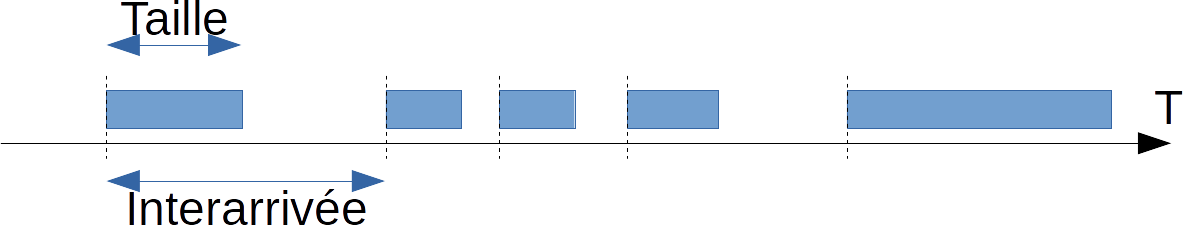
\includegraphics[width=0.5\textwidth]{trafic-base.png}
\caption{Modèle général d'une source\label{figure:trafic-base}}
\end{center}
\end{figure}

   Comme l'illustre la figure \ref{figure:trafic-base}, une source de
trafic sera caractérisé par deux composantes distinctes :
 
\begin{itemize}
   \item la loi régissant les dates de génération des paquets ;
   \item la loi régissant la taille des paquets.
\end{itemize}

   La modélisation d'une source dans un simulateur fondé sur {\sc
ndes} consiste donc en trois étapes de base : la création de la source
puis l'affectation des deux lois.

   Une source doit ensuite être démarrée pour produire des paquets.

   Le code complet de l'exemple décrit ici se trouve dans le fichier
{\tt trafic-model-ex.c} du répertoire {\tt examples}. Il peut donc
être compilé et exécuter de la façon suivante

\begin{verbatim}
 $ cd examples
 $ make trafic-model-ex
 $ ./trafic-model-ex
\end{verbatim}

   Le résultat est assez peu intéressant puisqu'il se contente
d'afficher le débit moyen de la source ! En revanche la lecture du
code est très intéressante ; enfin, pour peu qu'on s'intéresse à {\sc
  ndes} \ldots

%........................................................................
%
%........................................................................
\subsubsection{Création de la source}

   Nous allons définir puis créer une source de la façon suivante

\begin{verbatim}
#include <pdu-source.h>
   ...
   struct PDUSource_t  * sourcePDU;
   ...
   // We create the source and connect it to the sink
   sourcePDU = PDUSource_create(NULL,
                                sink,
                                (processPDU_t)PDUSink_processPDU);
\end{verbatim}

   Vous aurez remarqué que cette source envoie ici les paquets qu'elle
produit vers un puis. Notre but est en effet de focaliser uniquement
sur la source elle-même.

   Nous allons maintenant passer à la définition des lois
caractérisant cette source. Notons juste que dans les cas les plus
simples, cela peut également être réalisé simultanément à la création
en utilisant les fonctions décrites dans la section décrivant les
sources. 

%........................................................................
%
%........................................................................
\subsubsection{Définition de la loi des dates de départ}

   Chaque {\sc pdu} est généré à une date déterminée par une instance
de \lstinline!struct dateGenerator! défini dans {\tt
  include/date-generator.h}, dont il faut donc créer une instance.

   Mais avant ça, nous devons créer un générateur aléatoire  qui sera
utilisé par le générateur de date. En effet, les dates ne sont pas
générées directement, elles sont obtenue chacune par rapport à la
précédente par ajout d'une durée. C'est cette durée qui est fournie
par le générateur aléatoire.

   Imaginons que nous voulions simuler une source poissonienne de
paramètre $\lambda =10.0$, nous voulons un générateur d'inter-arrivé
exponentielle. Nous le créons donc de la façon suivante

\begin{verbatim}
#include <random-generator.h>
   ...
   struct randomGenerator_t * IARandGen; // The random generator for the source date generator
   ...
   double lambda = 10.0;
   ...
   // Initialisation of the interarrival random generator
   IARandGen = randomGenerator_createDoubleExp(lambda);
   ...
   // The date generator is characterised by the interarrival random
   // process
   dateGenerator_setRandomGenerator(dateGen, IARandGen);
\end{verbatim}

   Maintenant, nous pouvons créer le générateur de dates, auquel nous
affectons le générateur aléatoire ainsi créé, et que nous associons à
la source :

\begin{verbatim}
#include <date-generator.h>
   ...
   struct dateGenerator_t   * dateGen;   //!< The date generator for the source
   ...
   // Now, we want to define the packet creation process
   dateGen =  dateGenerator_create();
   ...
   // The date generator is characterised by the interarrival random
   // process
   dateGenerator_setRandomGenerator(dateGen, IARandGen);
   ...
   // Set the packet date generator
   PDUSource_setDateGenerator(sourcePDU, dateGen);
\end{verbatim}

%........................................................................
%
%........................................................................
\subsubsection{Définition de la loi des tailles}

   De la même façon que pour la loi d'inter arrivée, la loi de la
taille des {\sc pdu} doit être initialisée et associée à la source.
Cette loi est implantée par un générateur aléatoire que nous déclarons
ainsi :

\begin{verbatim}
#include <random-generator.h>
   ...
   struct randomGenerator_t * PSRandGen; // Packet size generator for the source
\end{verbatim}

   Nous allons ici générer des paquets dont la taille sera choisie
aléatoirement entre 4 valeurs équiprobables. Pour cela nous
définissons  les variables suivantes

\begin{verbatim}
#define nbSizes 4
   unsigned int sizes[nbSizes] = {
     128, 256, 512, 1024
   };
   double probas[nbSizes] = {
      0.25, 0.25, 0.25, 0.25
   };
\end{verbatim}

   Il ne nous reste plus qu'à initialier le générateur aléatoire (à
valeurs entières, bien sûr) et à l'associer à la source :

\begin{verbatim}
   // Creation of the packet size generator
   PSRandGen = randomGenerator_createUIntDiscreteProba(nbSizes, sizes, probas);

   // Set the packet size generator
   PDUSource_setPDUSizeGenerator(sourcePDU, PSRandGen);
\end{verbatim}

   Et voilà ! Notre source est prète à être utilisée. Si vous lancez
le programme fourni dans les exemples, vous constaterez en particulier
que le débit obtenu est d'environ 4 800 bit/seconde, ce qui
corrsespond bien aux valeurs utilisées ici (10 paquets par seconde de
taille moyenne 480 bits).

%------------------------------------------------------------------------
%
%------------------------------------------------------------------------
\subsection{Utilisation des sondes}

   Un simulateur réseau a pour vocation de permettre de réaliser des
mesures caractérisant les conditions de fonctionnement d'un modèle de
réseau (avec l'espoir que le modèle soit suffisament pertinent pour
que ces mesures soient applicables au réseau réel modélisé).

   Les outils de prise de mesure sont donc un élément important d'un
tel simulateur. Ce sont les sondes (ou {\em probes}) qui fournissent
un tel service dans {\sc ndes} ; elles sont décrites dans la section
\ref{section:sondes}.

   Le but de cet exemple est de montrer comment utiliser les sondes
pour une mesure plutôt classique en réseau : le débit.

\subsubsection{Mesurer un débit}

   Le programme d'exemple {\tt debits.c} montre plusieurs méthodes de
calcul d'un débit.

   Considérons le cas simple d'une source (comme celle de l'exemple
décrit dans la sous-section \ref{subsection:trafic-base}), dont nous
voulons mesurer le débit de sortie. Pour cela, nous allons insérer une
sonde sur la taille des paquets transmis grâce à la méthode {\tt
  PDUSource\_setPDUGenerationSizeProbe}.

   Le type de sonde dépendra de la mesure souhaitée.

%.......................................................................
%
%.......................................................................
\paragraph{Débit moyen}

   Supposons que nous voulons simplement connaître le débit moyen sur
toute la transmission, alors une sonde mesurant la moyenne sera parfaitement
suffisante :

%.......................................................................
%
%.......................................................................
\paragraph{Débit ``instantanté''}

